%! Author = kaliw
%! Date = 12/10/2019

% Convolutional Net
\subsection{The Convolutional Agent (aka Charizard)}

What we think will be our most evolved net, called Charizard, was created using a convolutional neural network.
The network architecture we use is:
\begin{itemize}
    \item Convolution 32@2x2
    \item Batch Normalization
    \item ReLU
    \item Convolution 64@2x2
    \item Batch Normalization
    \item ReLU
    \item Convolution 32@2x2
    \item Fully Connected 512x1
    \item Fully Connected 128x1
    \item Fully Connected 3x1
    \item Softmax
\end{itemize}
By trying a few different network architectures to see what would work best, we found that a very deep network did not suit a game such as tic-tac-toe.
The deeper networks that were tried took more time to compute and didn't return far superior results.

We used an Adam optimizer with $lr = 0.0001$, $\beta_1 = 0.9$ and $\beta_2 = 0.999$.
One thing that seemed interesting was that our training and validation accuracy didn't change very much after the first couple epochs.
We think part of the issue may be that without Monte Carlo Tree Search, using only random board states we don't see the best board states as frequently as we'd like and thus the network isn't learning as much about the best board states.
In a future iteration it would be nice to implement MCTS as well as a temporal dimension.

These are the results of the training runs:
\begin{figure}[h!]
	\centering
	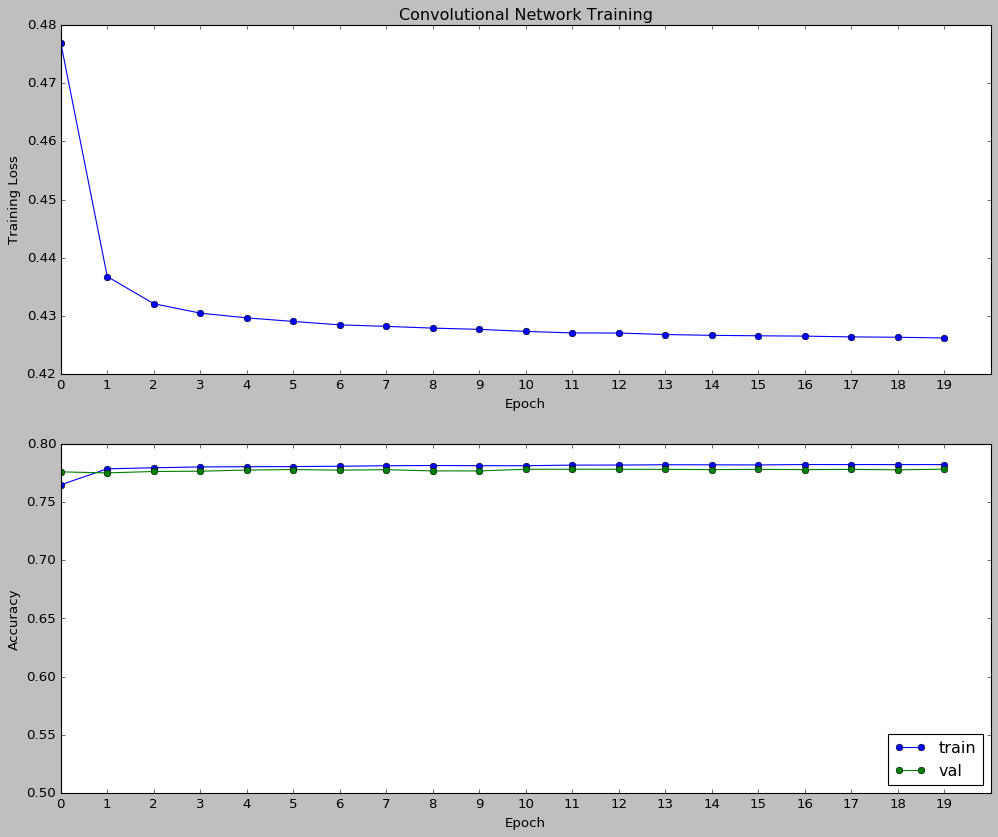
\includegraphics[width=10cm, height=7cm]{convolutional-net-training.png}
	\caption{Top: Training loss over 20 epochs.
    Bottom: Training accuracy against validation accuracy over 20 epochs}
	\label{fig:conv_net}
\end{figure}
